\documentclass[11pt]{article}

\usepackage{multicol}
\usepackage{graphicx}
\usepackage[english]{babel}
\usepackage[utf8]{inputenc}
\usepackage{amsmath}
\usepackage{amssymb}
\usepackage{listings}
\usepackage[numbered,framed]{matlab-prettifier}
\lstMakeShortInline"
\lstset{
  style              = Matlab-editor,
  %basicstyle         = \mlttfamily,
  escapechar         = ",
  mlshowsectionrules = true,
}

\newcommand{\buena}{[BUENA]}
\newcommand{\justifique}{[JUSTIFIQUE]}
\newcommand{\nojustifique}{[NOJUSTIFIQUE]}

\begin{document}
\title{C1_NUMERICO UDEC 2016-1}
\begin{itemize}
% \item Sean las instrucciones en código M
% \begin{lstlisting}
% A=ones(10);
% for i=2:10
% 	A=[A;diag(diag(A))]
% end
% A(:,end+1)=10;    
% \end{lstlisting}
% determine cual de las siguientes proposiciones es falsa
% \begin{enumerate} 
% \item\buena Al final de la ejecuci\'on la matriz A de orden $(80\times 80)$,
% \item Al final de la ejecuci\'on la la matriz A es de orden $10\times90$,
% \item Al final de la ejecuci\'on la primera fila de la matriz A tiene 18 veces el n\'umero 1.
% \item Al final de la ejecuci\'on la segunda columna de la matriz A tiene 10 veces el n\'umero 1.
% \end{enumerate}
% \nojustifique 

\item Dado $n\in\mathbb{N}$ arbitrario, se define
$$A=
\begin{bmatrix}
2 & 2 & \cdots & 2 \\
0 & 2 & \cdots & 2 \\
%0 & 0 & \ddots & 2 \\
\vdots&\vdots & \ddots& \vdots \\
0 & 0 & \cdots & 2
\end{bmatrix}_{n\times n},
$$
es decir una matriz triangular superior con elementos no nulos todos iguales a $2$. Se establecen sobre esta matriz las siguientes proposiciones
\begin{enumerate}
\item[i)] La matriz $A^tA$ es sim\'etrica.
\item[ii)] La matriz $A^t$ es triangular superior.
\item[iii)] $||A||_{1}=2n$
\item[iv)]	$||A||_{\infty}=2$
\end{enumerate}
Determine cual de estas proposiciones son verdaderas
\begin{enumerate} 
\item\buena S\'olo i) y iii)
\item S\'olo i)
\item S\'olo ii) y iv)
\item Ninguna de las anteriores.
\end{enumerate}
\nojustifique 

% \item Al final de la ejecuci\'on de las instrucciones 
% \begin{lstlisting}
% a=0;
% b=0;
% 	for i=1:10
%     a=a+0.1;
%     end
% if(a==1)
% 	b=1;
% end
% \end{lstlisting}
% la variable \texttt{b} vale cero.
% Determine cual de estas proposiciones son verdaderas
% \begin{enumerate} 
% \item Al final de la ejecuci\'on \texttt{a} es negativo.
% \item\buena Se comete un error por truncaci\'on en el c\'alculo de a.
% \item Todas las anteriores.
% \item Ninguna de las anteriores.
% \end{enumerate}
% \nojustifique 

\item Dado $c$ real fijo y los puntos
\begin{center}
\begin{tabular}{c|ccc}
x		& -2 & -3 & -1   \\
\hline
f(x)	& 0  & $c$  & 1 \\
\end{tabular}
\end{center}
Si 
$$
p(x)=\frac{-1}{2}(x+2)(3x+5)
$$
es el polinomio interpolante de estos puntos. Determine cual de estas proposiciones son verdaderas
\begin{enumerate} 
\item\buena $c=-2$,
\item El polinomio interpolante es una recta,
\item c=0.
\item $c=2$.
\end{enumerate}
\justifique 

\item Si $A$ es una matriz cuadradada que se puede factorizar LU sin pivoteo, entonces es cierto que 
\begin{enumerate} 
\item \buena $det(A)=det(U)$,
\item Si $A$ es no singular, entonces $U$ es singular,
\item $L$ es rectangular,
\item $det(A)=det(L)$.
\end{enumerate}
\justifique 

\item Si se sabe que el sistema $Ax=b$ se resuelve con una tolerancia de $10^{-8}$ con 25 iteraciones del método del gradiente conjugado. ¿Cu\'al de los siguientes gr\'aficos puede representar el error versus el número de iteraciones en la implementación de este algoritmo?. 
\begin{enumerate}
\item[i)]
\begin{centering}
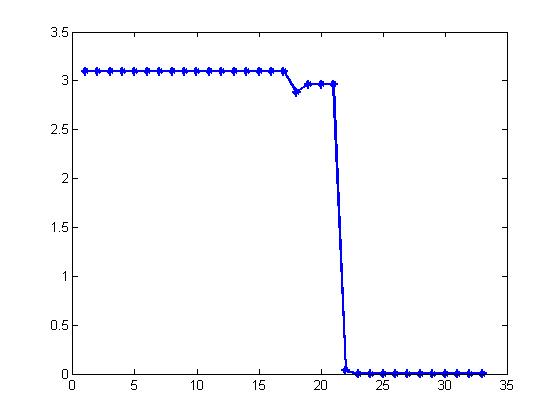
\includegraphics[width=0.8\textwidth]{p1.jpg}
\end{centering}
\item[ii)] 
\begin{centering}
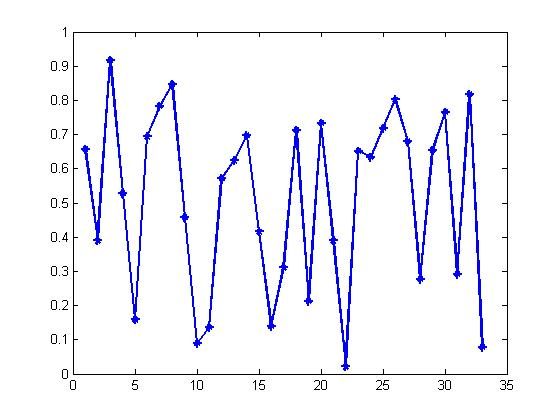
\includegraphics[width=0.8\textwidth]{p2.jpg}
\end{centering}
\item[iii)]
\begin{centering}
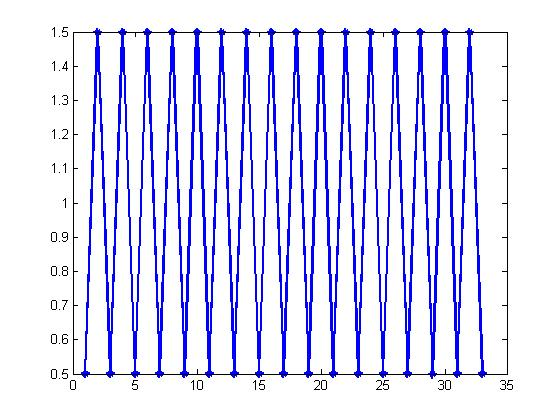
\includegraphics[width=0.8\textwidth]{p3.jpg}
\end{centering}
\item[iv)]
\begin{centering}
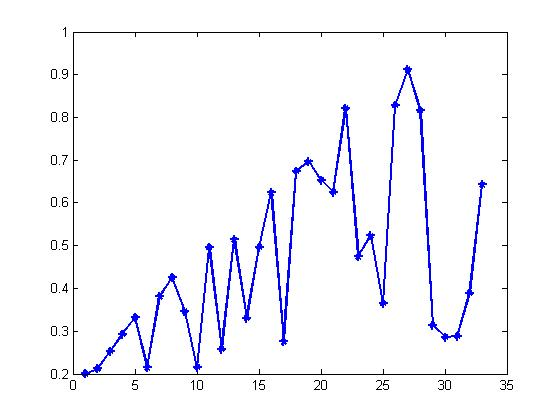
\includegraphics[width=0.8\textwidth]{p4.jpg}
\end{centering}
\end{enumerate}
\begin{enumerate} 
\item\buena S\'olo i)
\item S\'olo i) y ii)
\item S\'olo ii) y iv)
\item S\'olo iii)
\end{enumerate}
\nojustifique 

\end{itemize}
\end{document}